% Options for packages loaded elsewhere
\PassOptionsToPackage{unicode}{hyperref}
\PassOptionsToPackage{hyphens}{url}
%
\documentclass[
]{book}
\usepackage{amsmath,amssymb}
\usepackage{lmodern}
\usepackage{iftex}
\ifPDFTeX
  \usepackage[T1]{fontenc}
  \usepackage[utf8]{inputenc}
  \usepackage{textcomp} % provide euro and other symbols
\else % if luatex or xetex
  \usepackage{unicode-math}
  \defaultfontfeatures{Scale=MatchLowercase}
  \defaultfontfeatures[\rmfamily]{Ligatures=TeX,Scale=1}
\fi
% Use upquote if available, for straight quotes in verbatim environments
\IfFileExists{upquote.sty}{\usepackage{upquote}}{}
\IfFileExists{microtype.sty}{% use microtype if available
  \usepackage[]{microtype}
  \UseMicrotypeSet[protrusion]{basicmath} % disable protrusion for tt fonts
}{}
\makeatletter
\@ifundefined{KOMAClassName}{% if non-KOMA class
  \IfFileExists{parskip.sty}{%
    \usepackage{parskip}
  }{% else
    \setlength{\parindent}{0pt}
    \setlength{\parskip}{6pt plus 2pt minus 1pt}}
}{% if KOMA class
  \KOMAoptions{parskip=half}}
\makeatother
\usepackage{xcolor}
\usepackage{longtable,booktabs,array}
\usepackage{calc} % for calculating minipage widths
% Correct order of tables after \paragraph or \subparagraph
\usepackage{etoolbox}
\makeatletter
\patchcmd\longtable{\par}{\if@noskipsec\mbox{}\fi\par}{}{}
\makeatother
% Allow footnotes in longtable head/foot
\IfFileExists{footnotehyper.sty}{\usepackage{footnotehyper}}{\usepackage{footnote}}
\makesavenoteenv{longtable}
\usepackage{graphicx}
\makeatletter
\def\maxwidth{\ifdim\Gin@nat@width>\linewidth\linewidth\else\Gin@nat@width\fi}
\def\maxheight{\ifdim\Gin@nat@height>\textheight\textheight\else\Gin@nat@height\fi}
\makeatother
% Scale images if necessary, so that they will not overflow the page
% margins by default, and it is still possible to overwrite the defaults
% using explicit options in \includegraphics[width, height, ...]{}
\setkeys{Gin}{width=\maxwidth,height=\maxheight,keepaspectratio}
% Set default figure placement to htbp
\makeatletter
\def\fps@figure{htbp}
\makeatother
\setlength{\emergencystretch}{3em} % prevent overfull lines
\providecommand{\tightlist}{%
  \setlength{\itemsep}{0pt}\setlength{\parskip}{0pt}}
\setcounter{secnumdepth}{5}
\usepackage{booktabs}
\usepackage{amsthm}
\makeatletter
\def\thm@space@setup{%
  \thm@preskip=8pt plus 2pt minus 4pt
  \thm@postskip=\thm@preskip
}
\makeatother

\usepackage{tcolorbox}


\newtcolorbox{protip}{
  colback=black,
  coltext=white,
  colframe=black,
  boxsep=5pt,
  arc=4pt}
\newtcolorbox{bonus}{
  colback=blue!15,
  colframe=blue!15,
  coltext=black!80,
  boxsep=5pt,
  arc=4pt}
\newtcolorbox{reflect}{
  colback=green!5,
  colframe=green!5,
  coltext=black!80,
  boxsep=5pt,
  arc=4pt}
\newtcolorbox{assessment}{
  colback=blue!5,
  colframe=blue!5,
  coltext=black!80,
  boxsep=5pt,
  arc=4pt}
\newtcolorbox{progress}{
  colback=purple!10,
  colframe=purple!10,
  coltext=black!80,
  boxsep=5pt,
  arc=4pt}
\newtcolorbox{video}{
  colback=yellow!5,
  colframe=yellow!5,
  coltext=black!80,
  boxsep=5pt,
  arc=4pt}
\newtcolorbox{caution}{
  colback=red!5,
  colframe=red!5,
  coltext=black!80,
  boxsep=5pt,
  arc=4pt}
\newtcolorbox{feedback}{
  colback=black!5,
  colframe=black!5,
  coltext=black!80,
  boxsep=5pt,
  arc=4pt}
\newtcolorbox{todo}{
  colback=black!5,
  colframe=black!5,
  coltext=black!80,
  boxsep=5pt,
  arc=4pt}
\ifLuaTeX
  \usepackage{selnolig}  % disable illegal ligatures
\fi
\usepackage[]{natbib}
\bibliographystyle{apalike}
\IfFileExists{bookmark.sty}{\usepackage{bookmark}}{\usepackage{hyperref}}
\IfFileExists{xurl.sty}{\usepackage{xurl}}{} % add URL line breaks if available
\urlstyle{same} % disable monospaced font for URLs
\hypersetup{
  pdftitle={Presentations},
  pdfauthor={Colin Madland},
  hidelinks,
  pdfcreator={LaTeX via pandoc}}

\title{Presentations}
\author{Colin Madland}
\date{Last updated: 2023-03-09}

\begin{document}
\maketitle

{
\setcounter{tocdepth}{1}
\tableofcontents
}
\hypertarget{welcome}{%
\chapter*{Welcome}\label{welcome}}
\addcontentsline{toc}{chapter}{Welcome}

Please use the table of contents on the left to navigate through my presentations.

\hypertarget{otessa22---assessment-and-digital-technology-in-higher-education}{%
\chapter{OTESSA22 - Assessment and Digital Technology in Higher Education}\label{otessa22---assessment-and-digital-technology-in-higher-education}}

\hypertarget{introduction}{%
\section*{Introduction}\label{introduction}}
\addcontentsline{toc}{section}{Introduction}

\hypertarget{colin-madland-phd-candidate-university-of-victoria}{%
\subsection*{Colin Madland, PhD Candidate, University of Victoria}\label{colin-madland-phd-candidate-university-of-victoria}}
\addcontentsline{toc}{subsection}{Colin Madland, PhD Candidate, University of Victoria}

Slides - \url{https://bit.ly/otessa22-b}\\
\href{https://cmad.land}{Find me on the web\ldots{}}\\
\href{https://twitter.com/colinmadland}{Twitter}\\
\href{https://scholar.social/web/@Cmadland}{Mastodon}

\textbf{Presented Online at OTESSA22, May 17, 2022}

\begin{quote}
I acknowledge that the land where I currently live and work remains the traditional, ancestral, and unceded land of the \texttt{syilx} (silks) people, whose historical stewardship of and connections to the land continue to today. I am grateful to be an uninvited guest on this land. \href{https://wfn.ca}{To learn more, please visit the Westbank First Nation website.}
\end{quote}

\begin{figure}
\centering
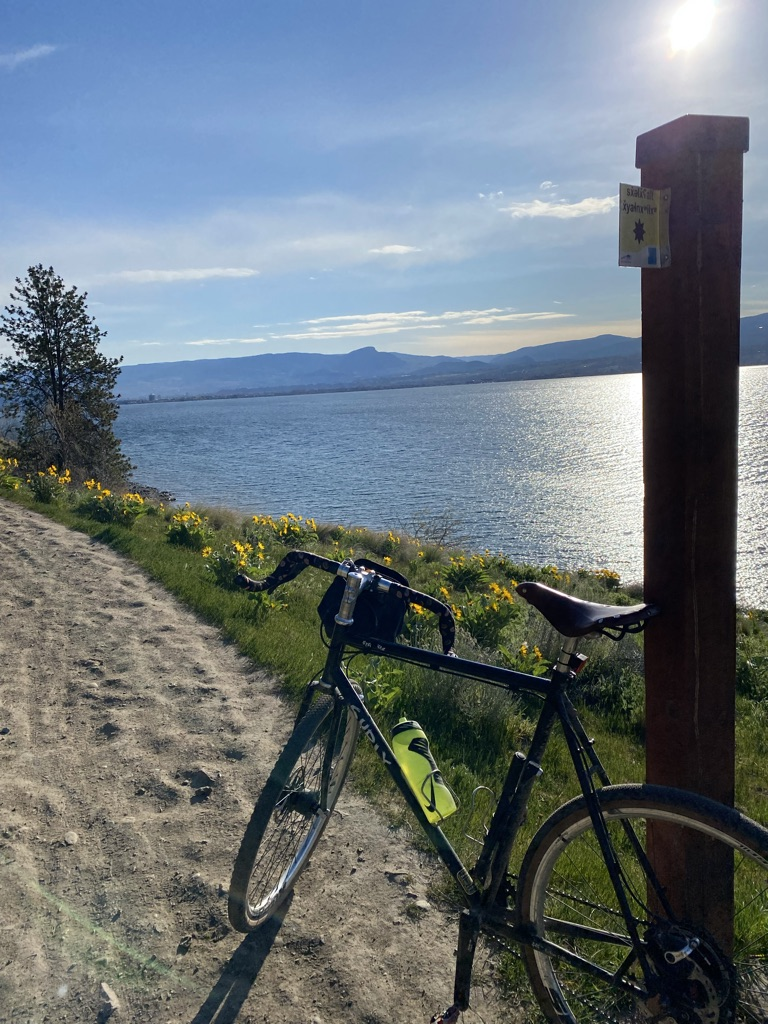
\includegraphics{assets/otessa22/kalamoir.jpg}
\caption{Figure 1. Author's bicycle overlooking Okanagan Lake.}
\end{figure}

\hypertarget{hypothes.is}{%
\subsection*{Hypothes.is}\label{hypothes.is}}
\addcontentsline{toc}{subsection}{Hypothes.is}

\href{https://web.hypothes.is/start/}{If you haven't already, feel free to sign up here as we will use hypothes.is later}. Also, if you have questions or comments, please annotate to your heart's content!

\hypertarget{background}{%
\subsection*{Background}\label{background}}
\addcontentsline{toc}{subsection}{Background}

This review is guided by four research questions:

\begin{enumerate}
\def\labelenumi{\arabic{enumi}.}
\tightlist
\item
  What are the major themes or patterns in the literature related to approaches to assessment in higher education?\\
\item
  What are the major themes or patterns in the literature related to the impact of technology on assessment in higher education?\\
\item
  What gaps exist in the literature related to approaches to assessment in technology-mediated higher education?
\end{enumerate}

\hypertarget{scriven-1967}{%
\subsubsection*{Scriven, 1967}\label{scriven-1967}}
\addcontentsline{toc}{subsubsection}{Scriven, 1967}

\begin{quote}
Scriven, M. (1967). \emph{The methodology of evaluation.} In B. O. Smith (Ed.), \emph{Perspectives of curriculum evaluation}. Rand McNally
\end{quote}

\begin{itemize}
\tightlist
\item
  distinction between \texttt{formative} and \texttt{summative}
\end{itemize}

\hypertarget{bloom-1968}{%
\subsubsection*{Bloom, 1968}\label{bloom-1968}}
\addcontentsline{toc}{subsubsection}{Bloom, 1968}

\begin{quote}
Bloom, B. (1968). Learning for Mastery. Instruction and Curriculum. Regional Education Laboratory for the Carolinas and Virginia, Topical Papers and Reprints, Number 1. \emph{Evaluation Comment, 1}(2), 12.
\end{quote}

\begin{itemize}
\tightlist
\item
  Incorporated \texttt{formative} and \texttt{summative} distinction into his ideas about \texttt{mastery\ learning}
\end{itemize}

\hypertarget{mislevy-1994}{%
\subsubsection*{Mislevy, 1994}\label{mislevy-1994}}
\addcontentsline{toc}{subsubsection}{Mislevy, 1994}

\begin{quote}
Mislevy, R. J. (1994). Test theory reconcieved. \emph{ETS Research Report Series, 1994}(1), i--38. \url{https://doi.org/10/gjm236}
\end{quote}

\begin{itemize}
\item
  \begin{quote}
  test theory is machinery for reasoning from students' behavior to conjectures about their competence, as framed in a particular conception of competence.''(p.~4).
  \end{quote}
\end{itemize}

\hypertarget{black-and-wiliam-1998}{%
\subsubsection*{Black and Wiliam, 1998}\label{black-and-wiliam-1998}}
\addcontentsline{toc}{subsubsection}{Black and Wiliam, 1998}

\begin{quote}
Black, P., \& Wiliam, D. (1998). Assessment and Classroom Learning. \emph{Assessment in Education: Principles, Policy \& Practice, 5}(1), 7--74. \url{https://doi.org/10/fpnss4}
\end{quote}

\begin{itemize}
\item
  major review of the literature on \texttt{formative\ assessment}\\
\item
  describe formative assessment as encouraging gains in achievement that were

\begin{verbatim}
> among the largest ever reported for educational interventions (p. 61)
\end{verbatim}
\end{itemize}

\hypertarget{pellegrino-et-al.-2001}{%
\subsubsection*{Pellegrino et al., 2001}\label{pellegrino-et-al.-2001}}
\addcontentsline{toc}{subsubsection}{Pellegrino et al., 2001}

\begin{quote}
Pellegrino, J. W., Chudowsky, N., \& Glaser, R. (2001). \emph{Knowing What Students Know: The Science and Design of Educational Assessment}. National Academies Press. \url{https://doi.org/10.17226/10019}
\end{quote}

\begin{itemize}
\tightlist
\item
  ``a process of drawing reasonable inferences about what students know on the basis of evidence derived from observations of what they say, do, or make in selected situations'' (p.~112)\\
\item
  ``reasoning from evidence'' (p.~43)
\end{itemize}

\hypertarget{assessment-triangle}{%
\paragraph*{Assessment Triangle}\label{assessment-triangle}}
\addcontentsline{toc}{paragraph}{Assessment Triangle}

\begin{figure}
\centering
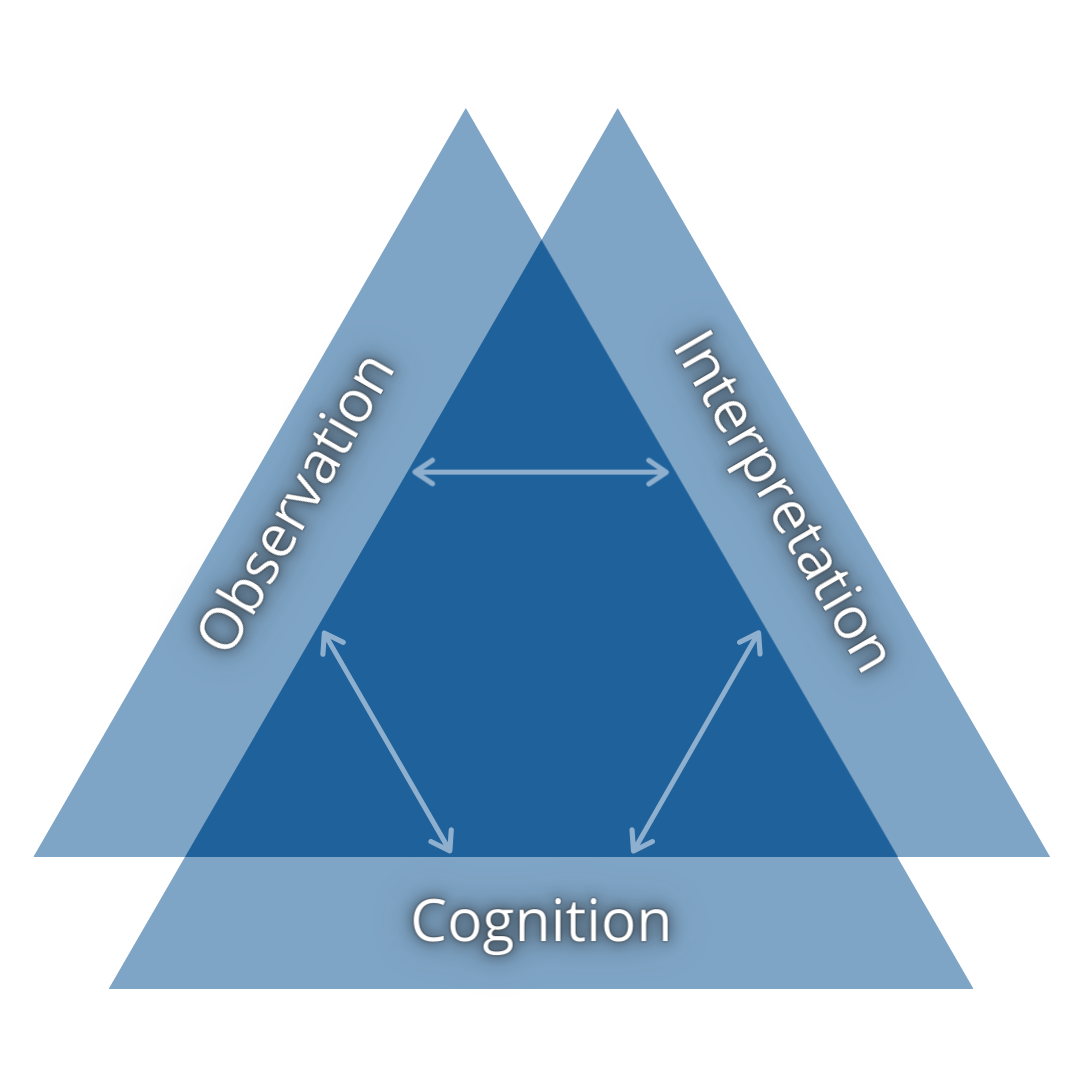
\includegraphics{assets/otessa22/assessment-triangle.png}
\caption{Figure 2. Assessment Triangle from Pellegrino et al.~(2001)}
\end{figure}

\hypertarget{cognition}{%
\subparagraph*{Cognition}\label{cognition}}
\addcontentsline{toc}{subparagraph}{Cognition}

\begin{itemize}
\tightlist
\item
  a cognitive model of the domain
\end{itemize}

\hypertarget{observation}{%
\subparagraph*{Observation}\label{observation}}
\addcontentsline{toc}{subparagraph}{Observation}

\begin{itemize}
\tightlist
\item
  a performance task used to gather data regarding learner achievement
\end{itemize}

\hypertarget{interpretation}{%
\subparagraph*{Interpretation}\label{interpretation}}
\addcontentsline{toc}{subparagraph}{Interpretation}

\begin{itemize}
\tightlist
\item
  an inference or judgement of the learner's achievement in relation to the model of the domain
\end{itemize}

\hypertarget{approaches-to-learning}{%
\subsection*{Approaches to Learning}\label{approaches-to-learning}}
\addcontentsline{toc}{subsection}{Approaches to Learning}

\hypertarget{biggs-1993}{%
\subsubsection*{Biggs, 1993}\label{biggs-1993}}
\addcontentsline{toc}{subsubsection}{Biggs, 1993}

\begin{quote}
Biggs, J. B. (1993). From Theory to Practice: A Cognitive Systems Approach. \emph{Higher Education Research \& Development, 12}(1), 73--85. \url{https://doi.org/10/ccdmd9}
\end{quote}

\begin{figure}
\centering
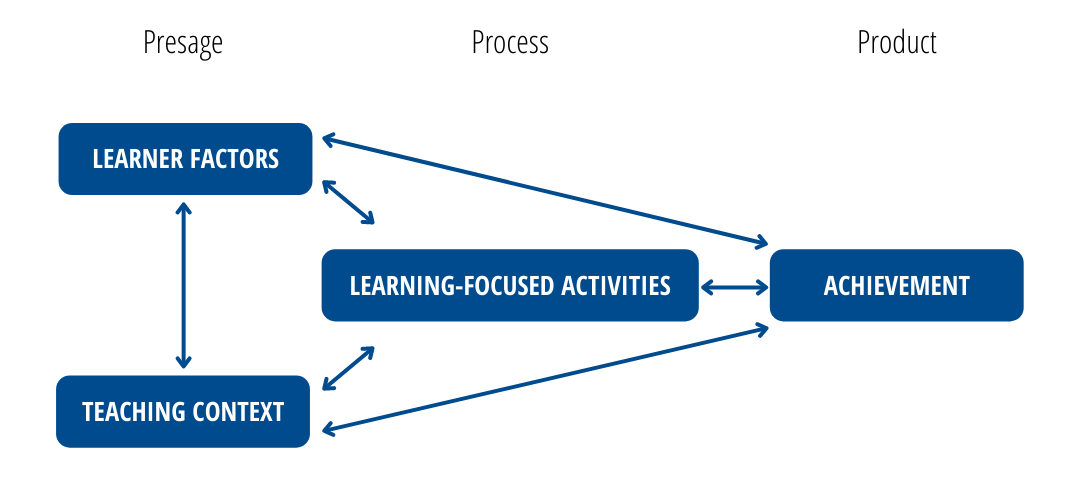
\includegraphics{assets/otessa22/3p-model.png}
\caption{Figure 3. 3-P Model of Teaching and Learning adapted from Biggs (1993)}
\end{figure}

\hypertarget{presage}{%
\paragraph*{Presage}\label{presage}}
\addcontentsline{toc}{paragraph}{Presage}

\begin{itemize}
\tightlist
\item
  factors that precede learning activities

  \begin{itemize}
  \tightlist
  \item
    learner factors

    \begin{itemize}
    \tightlist
    \item
      prior knowledge\\
    \item
      educational experience\\
    \item
      affective states\\
    \item
      wellness (physical \& mental)\\
    \end{itemize}
  \item
    teacher factors

    \begin{itemize}
    \tightlist
    \item
      vertical \& horizontal discourses (Bernstein, 1999)\\
    \item
      institutional policies\\
    \item
      department norms\\
    \item
      educational experiences
    \end{itemize}
  \end{itemize}
\end{itemize}

\hypertarget{process}{%
\paragraph*{Process}\label{process}}
\addcontentsline{toc}{paragraph}{Process}

\begin{itemize}
\tightlist
\item
  learning focused activities

  \begin{itemize}
  \tightlist
  \item
    reading, writing, discussing, building, creating, synthesizing, researching, sharing, debating, publishing\ldots{}
  \end{itemize}
\item
  surface approaches

  \begin{itemize}
  \tightlist
  \item
    using low-level cognitive skills when high-level cognitive skills are required
  \end{itemize}
\item
  deep approaches

  \begin{itemize}
  \tightlist
  \item
    using high-level cognitive skills for tasks which require them
  \end{itemize}
\end{itemize}

\hypertarget{product}{%
\paragraph*{Product}\label{product}}
\addcontentsline{toc}{paragraph}{Product}

\begin{itemize}
\tightlist
\item
  learner achievement of outcomes (intended or emergent)
\item
  fed back into the system

  \begin{itemize}
  \tightlist
  \item
    informs learners and instructors
  \end{itemize}
\end{itemize}

\hypertarget{conceptions-of-assessment}{%
\subsection*{Conceptions of Assessment}\label{conceptions-of-assessment}}
\addcontentsline{toc}{subsection}{Conceptions of Assessment}

\hypertarget{brown-1994-1996}{%
\subsubsection*{Brown, 1994; 1996}\label{brown-1994-1996}}
\addcontentsline{toc}{subsubsection}{Brown, 1994; 1996}

\begin{quote}
Brown, G. T. L. (2004). Teachers' conceptions of assessment: Implications for policy and professional development. \emph{Assessment in Education: Principles, Policy \& Practice, 11}(3), 301--318. \url{https://doi.org/10.1080/0969594042000304609}
\end{quote}

\begin{quote}
Brown, G. T. L. (2006). Teachers' Conceptions of Assessment: Validation of an Abridged Version. \emph{Psychological Reports, 99}(1), 166--170. \url{https://doi.org/10/bf67hf}
\end{quote}

\begin{itemize}
\tightlist
\item
  general mental structure, encompassing beliefs, meanings, concepts, propositions, rules, mental images, preferences

  \begin{itemize}
  \tightlist
  \item
    improvement of teaching and learning,\\
  \item
    school accountability,\\
  \item
    student accountability, or\\
  \item
    treating assessment as irrelevant.
  \end{itemize}
\end{itemize}

\hypertarget{fletcher-et-al.-2012}{%
\subsubsection*{Fletcher et al., 2012}\label{fletcher-et-al.-2012}}
\addcontentsline{toc}{subsubsection}{Fletcher et al., 2012}

\begin{quote}
Fletcher, R. B., Meyer, L. H., Anderson, H., Johnston, P., \& Rees, M. (2012). Faculty and Students Conceptions of Assessment in Higher Education. \emph{Higher Education, 64}(1), 119--133. \url{https://doi.org/10/ctccpq}
\end{quote}

\begin{itemize}
\tightlist
\item
  instructors were more likely than learners to view assessment as consistent and trustworthy methods to understand and improve learning\\
\item
  learners were more likely to have negative views of assessment and viewed it as a measure of student and institutional accountability.
\end{itemize}

\hypertarget{earl-2013}{%
\subsubsection*{Earl, 2013}\label{earl-2013}}
\addcontentsline{toc}{subsubsection}{Earl, 2013}

\begin{quote}
Earl, L. M. (2013). \emph{Assessment as learning: Using classroom assessment to maximize student learning (Second edition)}. Corwin Press.
\end{quote}

\begin{itemize}
\tightlist
\item
  Assessment \emph{OF} Learning

  \begin{itemize}
  \tightlist
  \item
    summative
  \end{itemize}
\item
  Assessment \emph{FOR} Learning

  \begin{itemize}
  \tightlist
  \item
    formative
  \end{itemize}
\item
  Assessment \emph{AS} Learning

  \begin{itemize}
  \tightlist
  \item
    metacognitive
  \end{itemize}
\end{itemize}

\hypertarget{approaches-to-assessment}{%
\subsection*{Approaches to Assessment}\label{approaches-to-assessment}}
\addcontentsline{toc}{subsection}{Approaches to Assessment}

Both learning and assessment are complex phenomena which are impacted by myriad factors.

\hypertarget{shepard-2000}{%
\subsubsection*{Shepard (2000)}\label{shepard-2000}}
\addcontentsline{toc}{subsubsection}{Shepard (2000)}

\begin{quote}
Shepard, L. A. (2000). The Role of Assessment in a Learning Culture. \emph{Educational Researcher, 29}(7), 4--14. \url{https://doi.org/10/cw9jwc}
\end{quote}

\begin{itemize}
\tightlist
\item
  traditional assessment structures originated in behaviourist models of teaching and learning

  \begin{itemize}
  \tightlist
  \item
    emphasis on culture of summative assessment
  \end{itemize}
\item
  modern constructivist models of teaching and learning are less compatible with previous assessment structures, yet a culture that emphasizes summative assessment seems to persist alongside emerging models of assessment
\end{itemize}

\hypertarget{deluca-2016}{%
\subsubsection*{DeLuca, 2016}\label{deluca-2016}}
\addcontentsline{toc}{subsubsection}{DeLuca, 2016}

\begin{quote}
DeLuca, C., LaPointe-McEwan, D., \& Luhanga, U. (2016). Approaches to classroom assessment inventory: A new instrument to support teacher assessment literacy. \emph{Educational Assessment, 21}, 248--266. \url{https://doi.org/10/gfgtsg}
\end{quote}

\begin{figure}
\centering
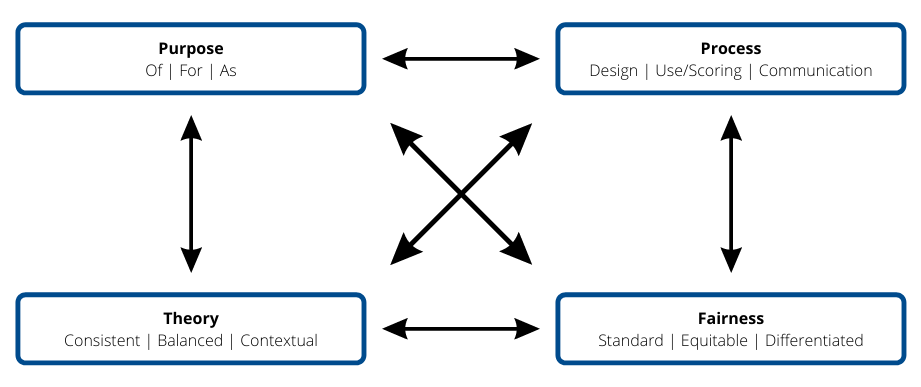
\includegraphics{assets/otessa22/approaches.png}
\caption{Figure 4. Approaches to Classroom Assessment from DeLuca et al.~(2016)}
\end{figure}

\begin{itemize}
\tightlist
\item
  \emph{Approaches to Classroom Assessment Inventory}

  \begin{itemize}
  \tightlist
  \item
    designed to inventory K12 teachers' thoughts, beliefs, actions related to assessment

    \begin{itemize}
    \tightlist
    \item
      Assessment purpose (of, for, as learning)\\
    \item
      Assessment process (design, use/scoring, communication)\\
    \item
      Assessment fairness (standard, equitable, differentiated)\\
    \item
      Assessment theory (consistent, balanced, contextual)
    \end{itemize}
  \end{itemize}
\end{itemize}

\hypertarget{technology-mediated-assessment-in-higher-education}{%
\section*{Technology-Mediated Assessment in Higher Education}\label{technology-mediated-assessment-in-higher-education}}
\addcontentsline{toc}{section}{Technology-Mediated Assessment in Higher Education}

\hypertarget{contrasting-with-k12}{%
\subsection*{Contrasting with K12}\label{contrasting-with-k12}}
\addcontentsline{toc}{subsection}{Contrasting with K12}

There is a very large body of literature on assessment in K12 learning contexts, and a not-quite as large, but still substantial body of literature on assessment in higher education. It may be tempting to conflate the two contexts, but K12 teachers typically complete 2 full years of pedagogical training as part of their academic and practical preparation. These two years often include specific courses on assessment, learning theory, as well as domain-specific pedagogies.

On the other hand, higher education instructors (from part-time sessionals to adjuncts to tenure-track and tenured faculty) tend to engage in little academic preparation in learning theories or assessment, although they seem to absorb the signature pedagogies of their discipline.

\hypertarget{impact-of-technology}{%
\subsection*{Impact of Technology}\label{impact-of-technology}}
\addcontentsline{toc}{subsection}{Impact of Technology}

\begin{itemize}
\tightlist
\item
  Impact on higher education is ubiquitous (SIS, LMS/VLE, CRM, etc.)
\item
  Tends to emphasize \texttt{efficiency} (however ill-defined that may be)

  \begin{itemize}
  \tightlist
  \item
    doing the same things with greater speed and/or reduced effort
  \item
    reinscribes mis-aligned assessment structures
  \end{itemize}
\end{itemize}

\hypertarget{pockets-of-innovation}{%
\subsubsection*{Pockets of Innovation}\label{pockets-of-innovation}}
\addcontentsline{toc}{subsubsection}{Pockets of Innovation}

\hypertarget{bearman-et-al.-2020}{%
\subsubsection*{Bearman et al.~2020}\label{bearman-et-al.-2020}}
\addcontentsline{toc}{subsubsection}{Bearman et al.~2020}

\begin{quote}
Bearman, M., Dawson, P., Ajjawi, R., Tai, J., \& Boud, D. (Eds.). (2020). \emph{Re-imagining university assessment in a digital world.} Springer.
\end{quote}

\begin{itemize}
\tightlist
\item
  cognitive offloading\\
\item
  artificial intelligence

  \begin{itemize}
  \tightlist
  \item
    ``personalized'' learning; recommender systems, automated item generation, automated essay scoring\\
  \end{itemize}
\item
  dialogic feedback

  \begin{itemize}
  \tightlist
  \item
    video, audio, screencast\\
  \end{itemize}
\item
  data \& learning analytics

  \begin{itemize}
  \tightlist
  \item
    process data\\
  \end{itemize}
\item
  peer/self-assessment
\item
  micro-credentials
\end{itemize}

However\ldots{}

\begin{itemize}
\tightlist
\item
  critical to consider ethical and social impacts!

  \begin{itemize}
  \tightlist
  \item
    surveillance
  \item
    equity
  \item
    algorithmic assessment
  \end{itemize}
\end{itemize}

\hypertarget{bower-2019}{%
\subsubsection*{Bower, 2019}\label{bower-2019}}
\addcontentsline{toc}{subsubsection}{Bower, 2019}

\begin{quote}
Bower, M. (2019). Technology‐mediated learning theory. \emph{British Journal of Educational Technology, 50}(3), 1035--1048. \url{https://doi.org/10.1111/bjet.12771}
\end{quote}

\begin{quote}
In technology-mediated learning contexts, agentic intentions reside with humans, and not with technology.
\end{quote}

\begin{itemize}
\tightlist
\item
  3 (select) premises

  \begin{itemize}
  \tightlist
  \item
    technology \texttt{mediates} between learners and outcomes\\
  \item
    beliefs, knowledge, practices, and environment are mutually influential (add this to the complexity of assessment)\\
  \item
    role of teachers is to optimise learning through the \texttt{purposeful\ deployment} of learning technologies
  \end{itemize}
\end{itemize}

\hypertarget{revisiting-shepard-2000}{%
\subsection*{Revisiting Shepard (2000)}\label{revisiting-shepard-2000}}
\addcontentsline{toc}{subsection}{Revisiting Shepard (2000)}

\textbf{Using hypothes.is}

\begin{itemize}
\tightlist
\item
  22 years have passed\ldots{}\\
\item
  What has changed?\\
\item
  What is your experience of technology-mediated assessment in higher education?\\
\item
  What are your greatest challenges related to technology-mediated assessment?
\end{itemize}

\hypertarget{themes-and-research-directions}{%
\section*{Themes and Research Directions}\label{themes-and-research-directions}}
\addcontentsline{toc}{section}{Themes and Research Directions}

\begin{itemize}
\tightlist
\item
  assessment as conversation in digital environments\\
\item
  validity exploration of \emph{Approaches to Assessment} in higher ed.\\
\item
  humanizing assessment, ethics
\end{itemize}

\hypertarget{questions-comments}{%
\section*{Questions? Comments?}\label{questions-comments}}
\addcontentsline{toc}{section}{Questions? Comments?}

\hypertarget{references}{%
\section*{References}\label{references}}
\addcontentsline{toc}{section}{References}

Bearman, M., Dawson, P., Ajjawi, R., Tai, J., \& Boud, D. (Eds.). (2020). \emph{Re-imagining university assessment in a digital world.} Springer.

Bernstein, B. (1999). Vertical and Horizontal Discourse: An Essay. \emph{British Journal of Sociology of Education, 20}(2), 157--173. JSTOR. \url{https://doi.org/10/ftmsvc}

Biggs, J. B. (1993). From Theory to Practice: A Cognitive Systems Approach. \emph{Higher Education Research \& Development, 12}(1), 73--85. \url{https://doi.org/10/ccdmd9}

Black, P., \& Wiliam, D. (1998). Assessment and Classroom Learning. \emph{Assessment in Education: Principles, Policy \& Practice, 5}(1), 7--74. \url{https://doi.org/10/fpnss4}

Bloom, B. (1968). Learning for Mastery. Instruction and Curriculum. Regional Education Laboratory for the Carolinas and Virginia, Topical Papers and Reprints, Number 1. \emph{Evaluation Comment, 1}(2), 12.

Bower, M. (2019). Technology‐mediated learning theory. \emph{British Journal of Educational Technology, 50}(3), 1035--1048. \url{https://doi.org/10.1111/bjet.12771}

Brown, G. T. L. (2004). Teachers' conceptions of assessment: Implications for policy and professional development. \emph{Assessment in Education: Principles, Policy \& Practice, 11}(3), 301--318. \url{https://doi.org/10.1080/0969594042000304609}

Brown, G. T. L. (2006). Teachers' Conceptions of Assessment: Validation of an Abridged Version. \emph{Psychological Reports, 99}(1), 166--170. \url{https://doi.org/10/bf67hf}

DeLuca, C., LaPointe-McEwan, D., \& Luhanga, U. (2016). Approaches to classroom assessment inventory: A new instrument to support teacher assessment literacy. \emph{Educational Assessment, 21}, 248--266. \url{https://doi.org/10/gfgtsg}

DeLuca, C., Willis, J., Cowie, B., Harrison, C., Coombs, A., Gibson, A., \& Trask, S. (2019). Policies, Programs, and Practices: Exploring the Complex Dynamics of Assessment Education in Teacher Education Across Four Countries. \emph{Frontiers in Education, 4}, 132. \url{https://doi.org/10/gh5k2r}

Earl, L. M. (2013). \emph{Assessment as learning: Using classroom assessment to maximize student learning (Second edition)}. Corwin Press.

Fletcher, R. B., Meyer, L. H., Anderson, H., Johnston, P., \& Rees, M. (2012). Faculty and Students Conceptions of Assessment in Higher Education. \emph{Higher Education, 64}(1), 119--133. \url{https://doi.org/10/ctccpq}

Mislevy, R. J. (1994). Test theory reconcieved. \emph{ETS Research Report Series, 1994}(1), i--38. \url{https://doi.org/10/gjm236}

Pellegrino, J. W., Chudowsky, N., \& Glaser, R. (2001). \emph{Knowing What Students Know: The Science and Design of Educational Assessment}. National Academies Press. \url{https://doi.org/10.17226/10019}

Scriven, M. (1967). \emph{The methodology of evaluation.} In B. O. Smith (Ed.), \emph{Perspectives of curriculum evaluation}. Rand McNally

Shepard, L. A. (2000). The Role of Assessment in a Learning Culture. \emph{Educational Researcher, 29}(7), 4--14. \url{https://doi.org/10/cw9jwc}

\hypertarget{twu-faculty-professional-learning}{%
\chapter{TWU Faculty Professional Learning}\label{twu-faculty-professional-learning}}

\textbf{Colin Madland, Manager, Online Learning and Instructional Technology (TWU GLOBAL) }

\emph{PhD Candidate, University of Victoria }

Notes - \url{https://bit.ly/twu-assessment}

\begin{figure}
\centering

\includegraphics{assets/twu-asmt/qr-slides.png}
\caption{QR Code to access presentation notes. You can scan the QR code with your mobile phone, then send the tab to your desktop (at least in FireFox).}
\end{figure}

\begin{itemize}
\tightlist
\item
  \href{https://cmad.land}{My web page}\\
\item
  \href{https://twitter.com/colinmadland}{Twitter}\\
\item
  \href{https://scholar.social/web/@Cmadland}{Mastodon}
\end{itemize}

\textbf{Presented Online for TWU Faculty Professional Learning, Thursday, March 9, 2023}

\begin{quote}
I acknowledge that the land where I currently live and work remains the traditional, ancestral, and unceded land of the \texttt{syilx} (silks) people, whose historical stewardship of and connections to the land continue to today. I am grateful to be an uninvited guest on this land. \href{https:/syilx.org}{To learn more, please visit the syilx.org.}
\end{quote}

\begin{figure}
\centering
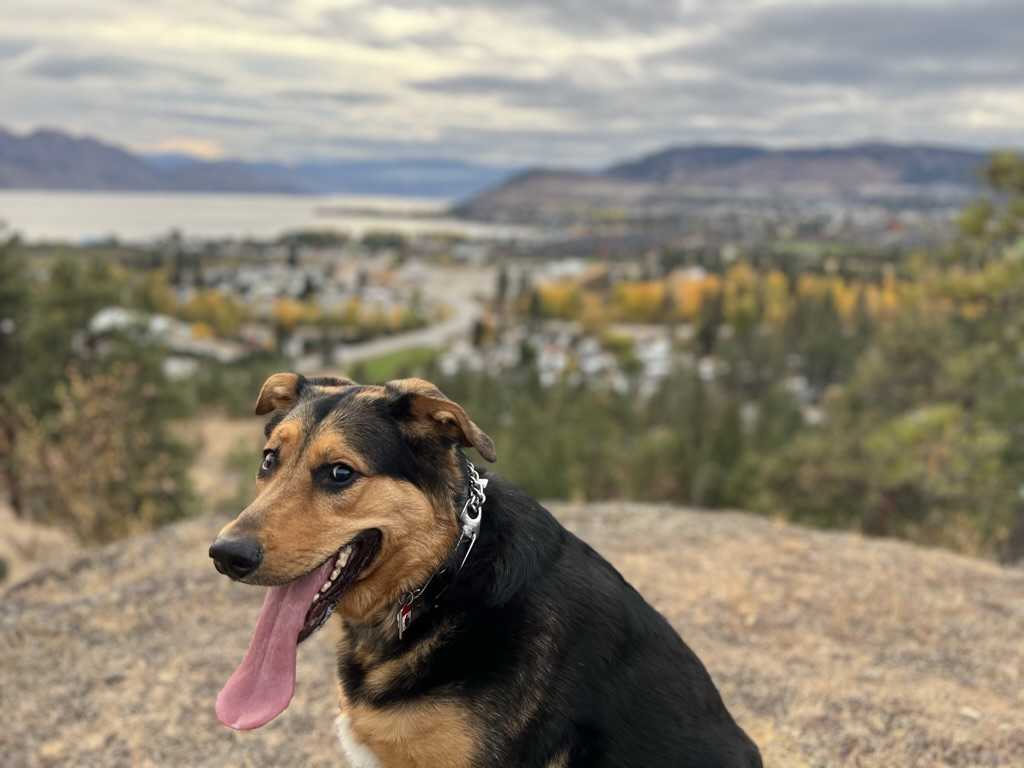
\includegraphics{assets/twu-asmt/ellie.jpeg}
\caption{My blind dog, Eleanor near the top of Mission Hill, overlooking syilx territory.}
\end{figure}

\hypertarget{what-is-assessment}{%
\section{What is `assessment'?}\label{what-is-assessment}}

\begin{figure}
\centering

\includegraphics{assets/twu-asmt/menti1.png}
\caption{QR Code to access Mentimeter}
\end{figure}

\textbf{Pellegrino, J. W., Chudowsky, N., \& Glaser, R. \href{https://doi.org/10.17226/10019}{\emph{Knowing What Students Know: The Science and Design of Educational Assessment}}. National Academies Press. }

\begin{quote}
``reasoning from evidence'' (p.~43)
\end{quote}

\begin{quote}
``a \textbf{\emph{process}} of drawing reasonable \textbf{\emph{inferences}} about what students know on the basis of \textbf{\emph{evidence}} derived from \textbf{\emph{observations}} of what they say, do, or make in \textbf{\emph{selected situations}}'' (p.~112)
\end{quote}

And a quote usually ascribed to Paul Dressel at various times and in various publications\ldots let me know if you find a verifiable source.

\begin{quote}
A grade is an inadequate report of an inaccurate judgment by a biased and variable judge of the extent to which a student has attained an undefined level of mastery of an unknown proportion of an indefinite material.
\end{quote}

\hypertarget{the-assessment-triangle}{%
\subsection{The Assessment Triangle}\label{the-assessment-triangle}}

\begin{figure}
\centering
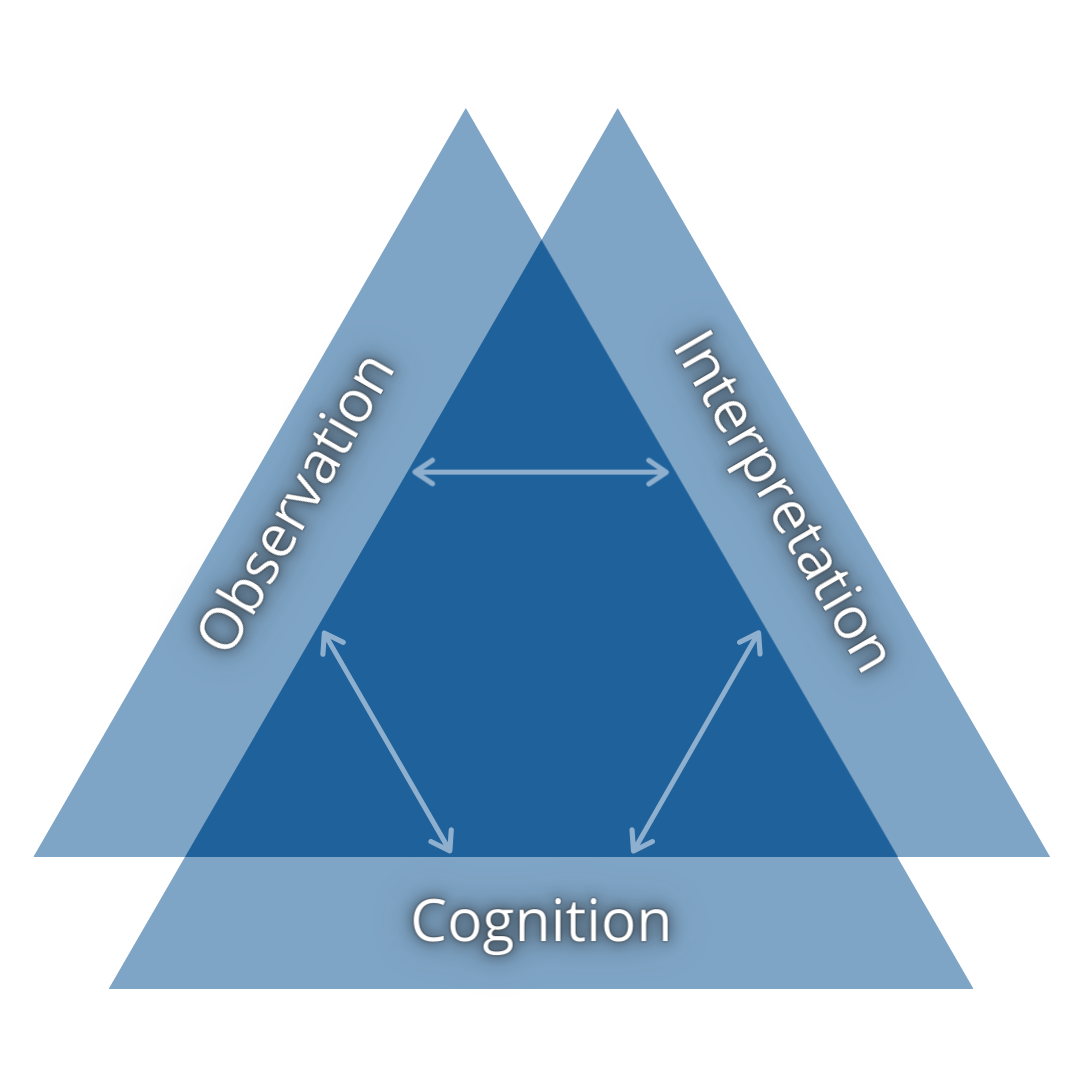
\includegraphics{assets/otessa22/assessment-triangle.png}
\caption{Assessment triangle showing the three components of assessment (Pellegrino, et al.~2001).}
\end{figure}

The process of assessment begins with a detailed understanding and map of the cognitive construct that is to be learned. This might be the ability to correctly calculate doses of medication, or transpose a piece of music, or write an argumentative essay. Below is an example of nursing competence from Weeks et al.~(2019).

\begin{figure}
\centering
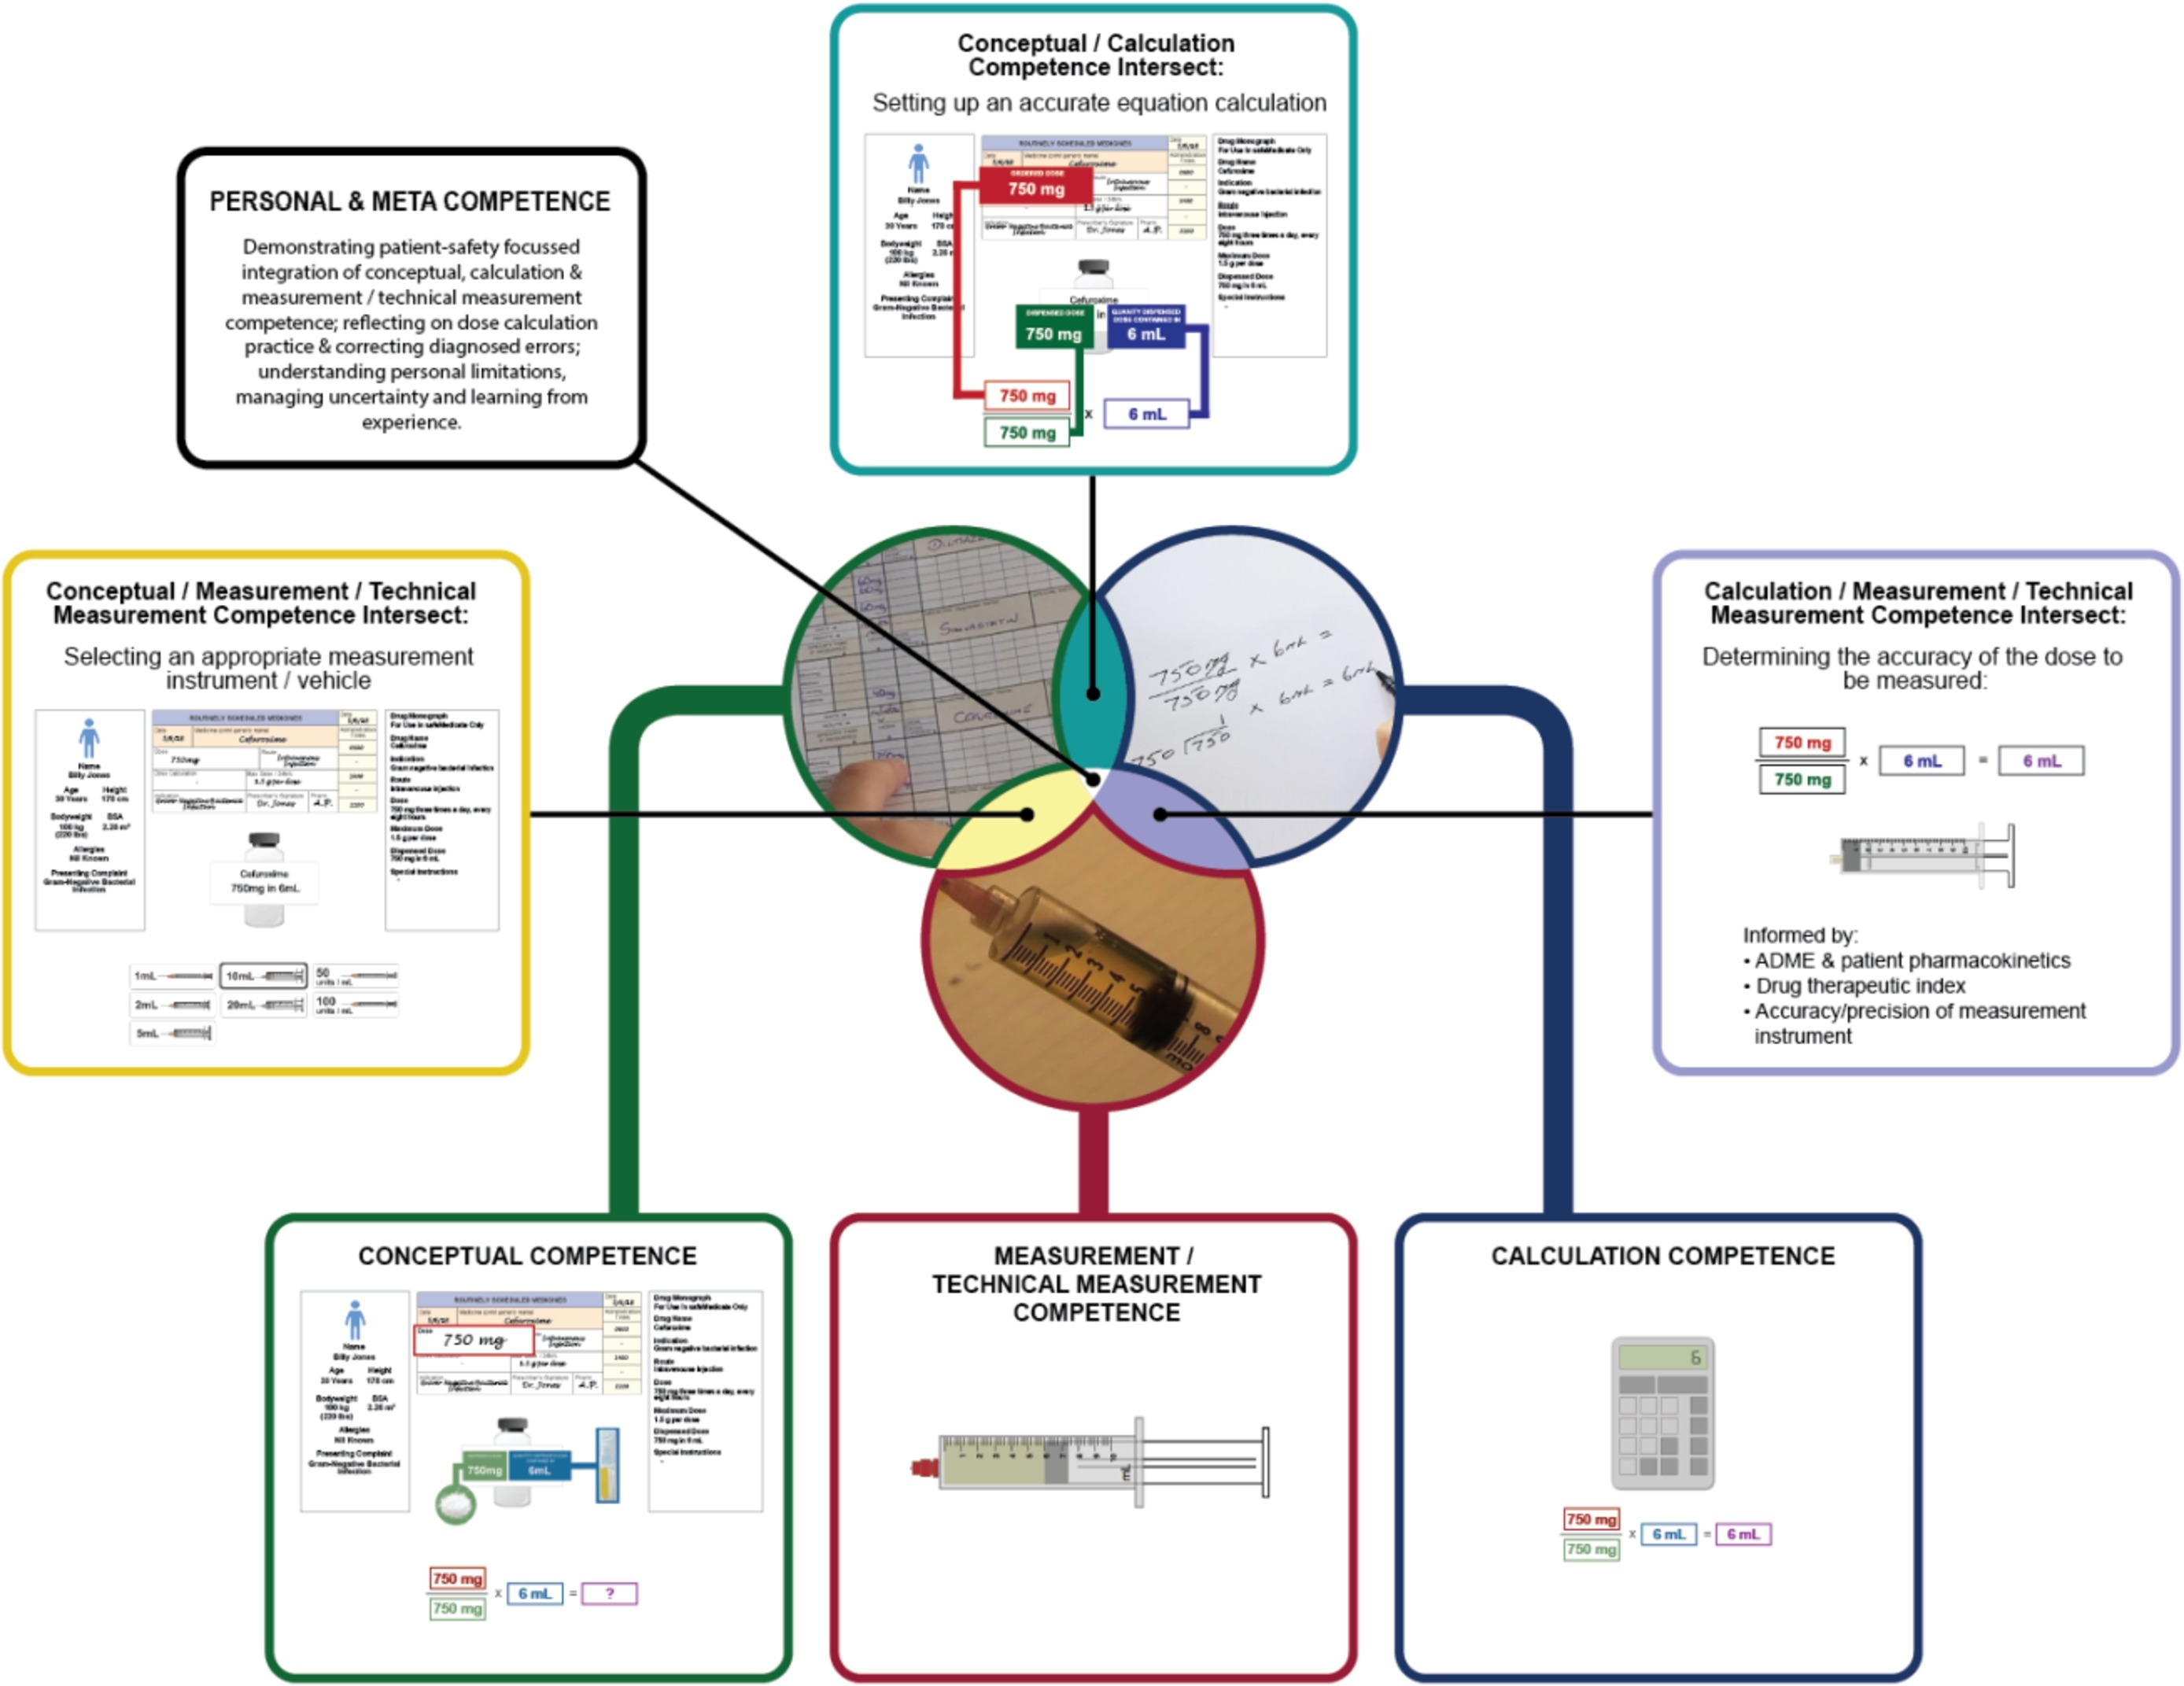
\includegraphics{assets/twu-asmt/nursing.jpg}
\caption{Drug dosage calculation competence from Weeks et al.~(2019)}
\end{figure}

Here are two documents in use in TWU Nursing. While these aren't constructed specifically as cognitive models of the domain, but instead as evaluation tools, the represent comprehesive models of what is required to demonstrate competency.

\begin{itemize}
\tightlist
\item
  \href{https://github.com/cmadland/decks/blob/main/assets/twu-asmt/mosby.pdf}{This is a checklist that nursing faculty use to allow learners to self-assess.}\\
\item
  \href{https://github.com/cmadland/decks/blob/main/assets/twu-asmt/n213.pdf}{And another used in practicum evaluations.}
\end{itemize}

The second component of the assessment triangle is an instrument of some kind designed to elicit the competencies mapped in the cognitive model. The instrument can vary widely from selected-response tests, videos, podcasts, performance tests in a lab, and many more.

The final component of assessment is an \emph{inference} or \emph{interpretation} of the data generated by the assessment instrument (not a \emph{measurement}). The accuracy of the interpretation depends on how well the instrument aligns with the cognitive model (validity) and how stable the results are across populations (reliability).

\begin{reflect}
One important thing to note is that many higher ed instructors (outside
of faculties of education or psychology) do not tend to have much formal
preparation in educational assessment, \emph{however}, higher education
instructors \emph{do} have extensive background and preparation for
conducting research. The assessment triangle above has many parallels to
research (cognitive model/literature review; instrument to gather data;
interpretation/discussion and conclusions).
\end{reflect}

\hypertarget{thinking-about-your-approach-to-assessment}{%
\section{Thinking about your Approach to Assessment}\label{thinking-about-your-approach-to-assessment}}

Scenario 1

\begin{quote}
You are teaching a large enrollment course. The students will be submitting bi-weekly assignments, a midterm exam, and a culminating assignment all designed to support their learning.
\end{quote}

\begin{enumerate}
\def\labelenumi{\arabic{enumi}.}
\tightlist
\item
  How would you approach grading the bi-weekly assignments?\\
\item
  How would you use data from learners' performance on the bi-weekly assignments?\\
\item
  How would you respond to learners who have diverse abilities in relation to the culminating assignment?\\
\item
  How would you deal with late assignments?
\end{enumerate}

\begin{figure}
\centering

\includegraphics{assets/twu-asmt/scenario1.png}
\caption{QR Code to access MentiMeter.}
\end{figure}

Scenario 2

\begin{quote}
A core assignment in your course involves students working in groups online.
\end{quote}

\begin{enumerate}
\def\labelenumi{\arabic{enumi}.}
\tightlist
\item
  How would you ensure accountability and engagement with the assignment?
\item
  How would you communicate feedback with the group?
\item
  What factors would you consider when making grading decisions?
\item
  How would you manage unexpected events that disrupt a group's ability to complete the assignment?
\end{enumerate}

\begin{figure}
\centering

\includegraphics{assets/twu-asmt/scenario2.png}
\caption{QR Code to access MentiMeter.}
\end{figure}

Scenario 3

\begin{quote}
There are expectations in your department that grades should be distributed across the grading scale. However, your class averages are consistently lower than your colleagues'. Your course assessment scheme includes two term exams and one final exam.
\end{quote}

\begin{enumerate}
\def\labelenumi{\arabic{enumi}.}
\tightlist
\item
  How might you incorporate assessment \emph{for} learning into your assessment scheme?
\item
  How might you design the exams to address the gap?
\item
  What would be a fair approach to `catching up' to your colleagues' course grades?
\item
  How might you analyze the exam scores to ensure reliability and validity?
\end{enumerate}

\begin{figure}
\centering

\includegraphics{assets/twu-asmt/scenario3.png}
\caption{QR Code to access MentiMeter.}
\end{figure}

Scenario 4

\begin{quote}
You teach a course with multiple sections taught by various instructors. Your students have complained to you that assignments are constructed and graded differently across sections.
\end{quote}

\begin{enumerate}
\def\labelenumi{\arabic{enumi}.}
\tightlist
\item
  How might different purposes of assessment (\ldots of/for/as learning) impact your response to learners?
\item
  What design strategies could mitigate the perception (or reality) of inconsistent assignments across sections?
\item
  What strategies could you use to ensure fairness across sections?
\item
  How might you ensure that your assignments are `measuring' the same things as your colleagues' assignments?
\end{enumerate}

\begin{figure}
\centering

\includegraphics{assets/twu-asmt/scenario4.png}
\caption{QR Code to access MentiMeter.}
\end{figure}

Scenario 5

\begin{quote}
You discover that a student has plagiarized some of their assignment (e.g., an essay, lab report).
\end{quote}

\begin{enumerate}
\def\labelenumi{\arabic{enumi}.}
\tightlist
\item
  How might your response change if the purpose of the assignment was one of assessment of/for/as learning?
\item
  How might you adjust the design or deployment of the assignment to reduce plagiarism?
\item
  What factors would you consider in deciding how to proceed with the student?
\item
  How can you come to know what the student knows in relation to the learning outcomes?
\end{enumerate}

\begin{figure}
\centering

\includegraphics{assets/twu-asmt/scenario5.png}
\caption{QR Code to access MentiMeter.}
\end{figure}

\hypertarget{a-framework-for-thinking-about-assessment}{%
\section{A Framework for Thinking about Assessment}\label{a-framework-for-thinking-about-assessment}}

\begin{figure}
\centering
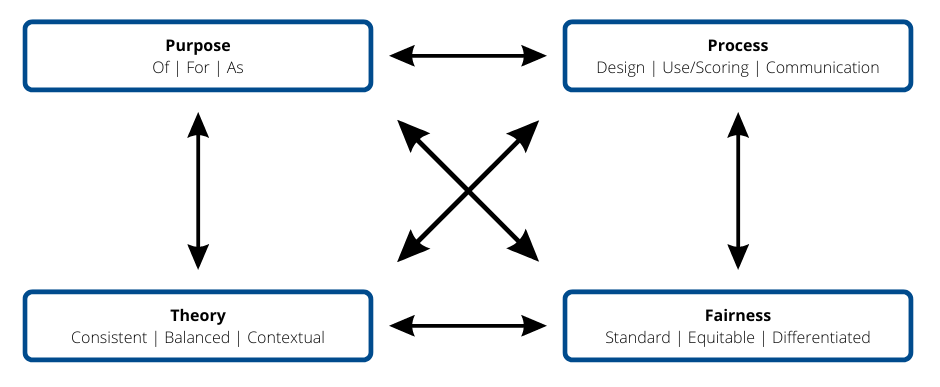
\includegraphics{assets/twu-asmt/approaches-2-assessment.png}
\caption{A Framework for Assessment as described below from DeLuca, et al.~(2016)}
\end{figure}

DeLuca et al.'s model for assessment comprises four dimensions, each with three priority themes. Each of these dimensions influence the other dimensions, and all influence instructors' approaches to assessment. The term `approaches to assessment' is intended to convey the reality that assessment in formal education is tremendously complex and idiosyncratic. Assessment literacy is not a checklist of competencies, `best' practices, or rules. The dimensions and their themes are listed below:

\begin{itemize}
\tightlist
\item
  Assessment Purpose

  \begin{itemize}
  \tightlist
  \item
    \ldots of learning\\
  \item
    \ldots for learning\\
  \item
    \ldots as learning\\
  \end{itemize}
\item
  Assessment Processes

  \begin{itemize}
  \tightlist
  \item
    design\\
  \item
    use and scoring\\
  \item
    communication\\
  \end{itemize}
\item
  Assessment Fairness

  \begin{itemize}
  \tightlist
  \item
    standard\\
  \item
    equitable\\
  \item
    balanced\\
  \end{itemize}
\item
  Measurement Theory

  \begin{itemize}
  \tightlist
  \item
    consistent\\
  \item
    balanced\\
  \item
    contextual
  \end{itemize}
\end{itemize}

\hypertarget{references-1}{%
\section*{References}\label{references-1}}
\addcontentsline{toc}{section}{References}

DeLuca, C., LaPointe-McEwan, D., \& Luhanga, U. (2016). \href{https://doi.org/10/gfgtsg}{Approaches to classroom assessment inventory: A new instrument to support teacher assessment literacy.} \emph{Educational Assessment, 21}, 248--266.

Pellegrino, J. W., Chudowsky, N., \& Glaser, R. (2001). \href{https://doi.org/10.17226/10019}{Knowing What Students Know: The Science and Design of Educational Assessment}. National Academies Press.

Weeks, K. W., Coben, D., O'Neill, D., Jones, A., Weeks, A., Brown, M., \& Pontin, D. (2019). \href{https://doi.org/10.1016/j.nepr.2019.04.010}{Developing and integrating nursing competence through authentic technology-enhanced clinical simulation education: Pedagogies for reconceptualising the theory-practice gap.} Nurse Education in Practice, 37, 29--38.

  \bibliography{book.bib}

\end{document}
